\documentclass{standalone}

\usepackage{tikz}

\begin{document}

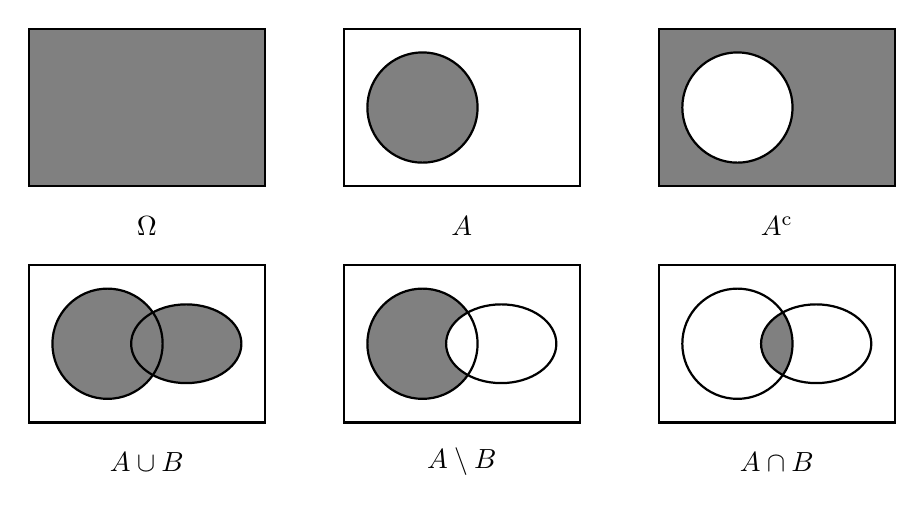
\begin{tikzpicture}
    \begin{scope}
        \draw[thick, fill=gray] (0, 0) rectangle (3, 2);
        \node at (1.5, -0.5) {$\Omega$};
    \end{scope}
    \begin{scope}[xshift=4cm]
        \draw[thick, fill=white] (0, 0) rectangle (3, 2);
        \draw[thick, fill=gray] (1, 1) circle (.7);
        \node at (1.5, -0.5) {$A$};
    \end{scope}
    \begin{scope}[xshift=8cm]
        \draw[thick, fill=gray] (0, 0) rectangle (3, 2);
        \draw[thick, fill=white] (1, 1) circle (.7);
        \node at (1.5, -0.5) {$A^{\mathrm{c}}$};
    \end{scope}
    \begin{scope}[yshift=-3cm]
        \draw[thick, fill=white] (0, 0) rectangle (3, 2);
        \fill[gray] (1, 1) circle (.7) (2, 1) ellipse (.7 and .5);
        \draw[thick] (1, 1) circle (.7);
        \draw[thick] (2, 1) ellipse (.7 and .5);
        \node at (1.5, -0.5) {$A\cup B$};
    \end{scope}
    \begin{scope}[yshift=-3cm, xshift=4cm]
        \draw[thick, fill=white] (0, 0) rectangle (3, 2);
        \fill[gray] (1, 1) circle (.7);
        \draw[thick, fill=white] (2, 1) ellipse (.7 and .5);
        \draw[thick] (1, 1) circle (.7);
        \node at (1.5, -0.5) {$A\setminus B$};
    \end{scope}
    \begin{scope}[yshift=-3cm, xshift=8cm]
        \draw[thick, fill=white] (0, 0) rectangle (3, 2);
        \begin{scope}
            \clip (1, 1) circle (.7);
            \fill[gray] (2, 1) ellipse (.7 and .5);
        \end{scope}
        \draw[thick] (1, 1) circle (.7);
        \draw[thick] (2, 1) ellipse (.7 and .5);
        \node at (1.5, -0.5) {$A\cap B$};
    \end{scope}
\end{tikzpicture}

\end{document}